% %
% LAYOUT_E.TEX - Short description of REFMAN.CLS
%                                       99-03-20
%
%  Updated for REFMAN.CLS (LaTeX2e)
%
%\documentclass[a4paper]{refart}
\documentclass[a4paper]{article}
%\usepackage{makeidx}
%\usepackage{ifthen}
\usepackage{lipsum}
\usepackage{afterpage}
\usepackage{graphicx}

% ifthen wird vom Bild von N.Beebe gebraucht!

\def\bs{\char'134 } % backslash in \tt font.
\newcommand{\ie}{i.\,e.,}
\newcommand{\eg}{e.\,g..}
\DeclareRobustCommand\cs[1]{\texttt{\char`\\#1}}
\usepackage{listings}

\lstset{
basicstyle=\small\ttfamily,
columns=flexible,
breaklines=true
}

\title{glactools: a suite of utilities for the management of allele frequency information}
\author{Gabriel Renaud \\
gabriel [dot] reno [at]  gmail.com}

\date{}
%\emergencystretch1em  %

%\pagestyle{myfootings}
%\markboth{Changing the layout with \textrm{\LaTeX}}%
%         {Changing the layout with \textrm{\LaTeX}}

\makeindex 

%\setcounter{tocdepth}{2}


\usepackage{filecontents}
\begin{filecontents}{bibli.bib}
@article{prufer2010computational,
  title={Computational challenges in the analysis of ancient {D}{N}{A}},
  author={Pr{\"u}fer, Kay and Stenzel, Udo and Hofreiter, Michael and P{\"a}{\"a}bo, Svante and Kelso, Janet and Green, Richard E},
  journal={Genome {B}iology},
  volume={11},
  number={5},
  pages={R47},
  year={2010},
  publisher={BioMed Central Ltd}
}

@article{wilson1927probable,
  title={Probable inference, the law of succession, and statistical inference},
  author={Wilson, Edwin B},
  journal={{J}ournal of the {A}merican {S}tatistical {A}ssociation},
  volume={22},
  number={158},
  pages={209--212},
  year={1927},
  publisher={Taylor \& Francis Group}
}

@article{patterson2012ancient,
  title={{A}ncient admixture in human history},
  author={Patterson, Nick and Moorjani, Priya and Luo, Yontao and Mallick, Swapan and Rohland, Nadin and Zhan, Yiping and Genschoreck, Teri and Webster, Teresa and Reich, David},
  journal={Genetics},
  volume={192},
  number={3},
  pages={1065--1093},
  year={2012},
  publisher={Genetics Soc America}
}

\end{filecontents}
\usepackage{natbib}

\begin{document}

\maketitle

\begin{abstract}
glactools is a set of command-line utilities to store genotype likelihoods and allele count data. It can import data from various formats, merge/filter/split datasets, compute summary statistics and exporting data to various formats.
\end{abstract}

\tableofcontents


\section{Introduction}

glactools aims at storing either :
\begin{itemize}
\item genotype likelihoods for a single diploid individual for autosomal data (GLF format).
\item allele count information for either a given individual or population (ACF format)
\end{itemize}
imported from various input sources (VCF, BAM etc), creating intersections, querying the data and exporting it to various formats used by current software tools.

\subsection{Installation}

Please refer to the README for downloading and installing the software.




\noindent \begin{tabular}{|l|l|}
\hline
Program & Use \\
\hline
\multicolumn{2}{|l|}{Data import} \\
\hline
      vcf2acf     &    Convert single sample VCF to acf  \\
      vcf2glf     &    Convert single sample VCF to glf  \\
      vcfm2acf    &    Convert multi  sample VCF to acf  \\
      bam2acf     &    Convert single sample BAM to acf  \\
      axt2acf     &    Convert AXT alignment to acf  \\
      23andme2acf &    Convert 23andme data to acf  \\
\hline
\multicolumn{2}{|l|}{Filtering} \\
\hline
      noundef     &    No undefined sites for populations \\
      bedfilter   &    Filter ACF/GLF file using sorted bedfile \\
      segsite     &    Just retain segregating sites (or trans./transi) \\
      sharing     &    Retain sites that share alleles between populations \\
      nosharing   &    Retain sites that do NOT share alleles between populations \\
      snosharing  &    Retain sites that STRICKLY do NOT share alleles between populations \\
\hline
\multicolumn{2}{|l|}{Computations} \\
\hline
      freqspec    &    Compute the frequency spectrum \\
      closest     &    Return the distance between records \\
      compute     &    Compute summary statistics \\
      stats       &    Provide very basic stats \\
\hline
\multicolumn{2}{|l|}{File transformations} \\
\hline
      cat         &    Concatenate (GL|AC)f files \\
      intersect   &    Intersection of (GL|AC)f files \\
      union       &    Union of (GL|AC)f files \\
      reheader    &    Replace header of (GL|AC)f files \\
\hline
\multicolumn{2}{|l|}{Population transformations} \\
\hline
      meld        &    Merge multiple populations as one for ACF files \\
      popsub      &    Keep a subset of the populations \\
      removepop   &    Remove a subset of the populations \\
      replaceanc  &    Use ancestral/root information from another file \\
      usepopsrootanc &  Use 2 specified pops as ancestral/root information \\
      rename      &    Rename populations \\
\hline
\multicolumn{2}{|l|}{Data export} \\
\hline
      glac2bed    &    Convert a (GL|AC)f file to BED \\
      acf2bplink  &    Convert an ACF file to binary PLINK \\
      acf2fasta   &    Convert an ACF file to fasta \\
      acf2gphocs  &    Convert an ACF file to G-PhoCs \\
      acf2nexus   &    Convert an ACF file to Nexus \\
      acf2treemix &    Convert an ACF file to treemix \\
      acf2eigenstrat &  Convert an ACF file to EIGENSTRAT \\
\hline
\multicolumn{2}{|l|}{GLF/ACF conversion} \\
\hline
      glf2acf     &    Convert glf to acf  \\
\hline
\multicolumn{2}{|l|}{Indexing} \\
\hline
      index       &    Index acf/glf file \\
      idxstats    &    Basic statistics using the index of a acf/glf file \\
\hline
\multicolumn{2}{|l|}{Viewing}\\ 
\hline
      view        &    View all or a region of a ACF/GLF file  \\
\hline
\end{tabular}

\section{File format}


\noindent  A glactools file can be 2 types of files:
\begin{itemize}
\item {\bf GLF}: genotype likelihoods file for a single diploid individual individual
\item {\bf ACF}: allele count file for 1 or more indivuals
\end{itemize}

\noindent  Each one of these files can either be:
\begin{itemize}
\item {\bf binary and bgzipped}: Default output. Recommended as it saves space and can be indexed
\item {\bf binary}:  only used for UNIX pipes into another program
\item {\bf text and (bg)zipped}: 
\item {\bf text}: not recommend as it waste disk space
\end{itemize}

\noindent In addition to containing the fields for the various populations/individuals, the format  has also 2 special fields to contain a root population and an ancestral population.  The route population (labeled  ``root'') corresponds to some outgroup to all other individuals (e.g. chimp for humans).  The ancestral population (labeled  ``anc'')  corresponds to the most recent common ancestor of all the individuals in the ACF or GLF file and the root population (e.g. chimp/human ancestor for humans).
\subsection{Text format}


When stored as a text file (zipped or not), a glactools file a composed of a header and the data. Each line in the header starts with a \# and has different slightly formats for a GLF/ACF files.

\subsubsection{GLF} 
\label{text:glf}
\noindent The header has the following format

\begin{lstlisting}
#GLF
#PG:[command line used]
#GITVERSION: [github revision]
#DATE: YYYY-MM-DD
#[PROGRAM TAG]
#SQ     SN:[FIRST  CHROMOSOME]    LN:[FIRST  CHROMOSOME LENGTH]
#SQ     SN:[SECOND CHROMOSOME]    LN:[SECOND CHROMOSOME LENGTH]
...
#SQ     SN:[LAST   CHROMOSOME]    LN:[LAST   CHROMOSOME LENGTH]
#chr    coord   REF,ALT root    anc     pop1     pop2     ...
\end{lstlisting}


\noindent The lines starting with {\bf \#SQ} define the chromosomes of the reference and their lengths. The line starting with {\bf \#chr} is called the defline as it contains the name of the individuals. The following lines:

\begin{lstlisting}
#SQ     SN:[LAST   CHROMOSOME]    LN:[LAST   CHROMOSOME LENGTH]
#chr    coord   REF,ALT root    anc     pop1     pop2     ...
\end{lstlisting}

\noindent use a [tab] to separate the fields. 

\noindent \textbf{Genotype likelihoods}
\noindent The remaining lines contain the actual data have the following format:

\begin{lstlisting}
chr    coord   REF,ALT [root info]     [anc info]     [pop1 info]     [pop2 info]     ...
\end{lstlisting}

\noindent  Each field is [TAB] delimited. The ALT allele is set to N if there were no alternative allele found. The info for GLF has the following format:

\begin{lstlisting}
[ref,ref GL],[ref,alt GL],[alt,alt GL]:[CPG flag 0=no,1=yes]
\end{lstlisting}

\noindent where GL=genotype likelihoods and is on a PHRED scale and between 0..255. Here is an example of valid lines:

\begin{lstlisting}
1	1689574	A,N	0,255,255:0	0,255,255:0	0,45,120:0
1	1689575	T,C	255,0,255:0	0,255,255:0	0,25,90:0
\end{lstlisting}

\subsubsection{ACF} 

\label{text:acf}
\noindent The header has the following format:

\begin{lstlisting}
#ACF
#PG:[command line used]
#GITVERSION: [github revision]
#DATE: YYYY-MM-DD
#[PROGRAM TAG]
#SQ     SN:[FIRST  CHROMOSOME]    LN:[FIRST  CHROMOSOME LENGTH]
#SQ     SN:[SECOND CHROMOSOME]    LN:[SECOND CHROMOSOME LENGTH]
...
#SQ     SN:[LAST   CHROMOSOME]    LN:[LAST   CHROMOSOME LENGTH]
#chr    coord   REF,ALT root    anc     pop1     pop2     ...
\end{lstlisting}


\noindent The lines starting with  SQ define the chromosomes of the reference and their lengths. The line starting with chr is called the defline as it contains the name of the individuals. The following lines:

%\noindent The lines starting with {\texttt \#SQ } define the chromosomes of the reference and their lengths. The line starting with {\texttt \#chr} is called the defline as it contains the name of the individuals/populations. The following lines:

\begin{lstlisting}
#SQ     SN:[LAST   CHROMOSOME]    LN:[LAST   CHROMOSOME LENGTH]
#chr    coord   REF,ALT root    anc     pop1     pop2     ...
\end{lstlisting}

\noindent use a [tab] to separate the fields. 

\noindent \textbf{Allele counts}
\noindent The remaining lines contain the actual data have the following format:

\begin{lstlisting}
chr    coord   REF,ALT [root info]     [anc info]     [pop1 info]     [pop2 info]     ...
\end{lstlisting}

\noindent  The ALT allele is set to N if there were no alternative allele found. The info for GLF has the following format:

\begin{lstlisting}
[REF allele count],[ALT allele count]:[CPG flag 0=no,1=yes]
\end{lstlisting}

\noindent  The allele counts are raw counts and between 0..65535. Here is an example of valid lines:

\begin{lstlisting}
1	1689574	A,N	1,0:0	1,0:0	2,0:0
1	1689575	T,C	0,1:0	1,0:0	2,0:0
\end{lstlisting}



\subsection{Binary}


\noindent The binary format has the following specifications. We recommend to store the format as a binary bgzip file as it can be indexed easily. However for UNIX piping we recommend to use the uncompressed version (option -u). An ACF/GLF file in binary format has the following format:

%\begin{table}

\noindent \begin{tabular}{|l|p{5cm}|l|l|}
\hline
{\bf Field} & {\bf Description} & {\bf Type} & {\bf Value} \\
\hline
bammagicstr & BAM magic string. This field has no purporse but to make htslib happy & char [4] & BAM\textbackslash1 \\
\hline
magicstr & ACF/GLF magic string. This field indicates whether this file is in GLF or ACF format & char [5] & ACF2\textbackslash1 or \\
         &  It is either ACF or GLF followed by the number of bytes per record (1 for GLF 2 for ACF)   &          & GLF1\textbackslash1 \\
         &  Currently, the code support up to 65535 alleles but could be extended for higher numbers   &          &  \\
\hline
sizeheader & size of the header in bytes   & uint32\_t         & \\
\hline
header     & The header (see section \ref{text:glf} and \ref{text:acf}) in bytes           & char [sizeheader] & \\
\hline
sizePops   & The number of populations {\bf excluding}  the root and anc & uint32\_t         & \\
% \multic
\hline
\multicolumn{4}{|c|}{Begin list of records} \\
\hline
\multicolumn{1}{|c|}{chri}   & The index of the chromosome & uint16\_t         & \\
\hline
\multicolumn{1}{|c|}{coordinate}   & The coordinate on the chromosome & uint32\_t         & \\
\hline
\multicolumn{1}{|c|}{REF$\vert$ALT}     & The first 4 bits are for the REF, the last for the ALT & uint8\_t         & \\
                                & N=0000, A=0001, C=0010, G=0011, T=0100                  &          & \\
\hline
\multicolumn{4}{|c|}{Begin list of individuals/populations (see below)} \\
\hline
\end{tabular}
%\end{table}

\afterpage{\clearpage}


\subsubsection{GLF}

\noindent Each record contains the following for (sizePops+2) times:

%\begin{table}
\noindent \begin{tabular}{|r|p{6cm}|l|l|}
\hline
{\bf Field} & {\bf Description} & {\bf Type} & {\bf Value} \\
\hline
rrGL & Genotype likelihood on a PHRED scale for the ref,ref genotype & uint8\_t &  \\
\hline
raGL & Genotype likelihood on a PHRED scale for the ref,alt genotype & uint8\_t &  \\
\hline
aaGL & Genotype likelihood on a PHRED scale for the alt,alt genotype & uint8\_t &  \\
\hline
CpG & Flag to know whether the actual individual is a CpG or not & uint8\_t &  \\
\hline
\end{tabular}
%\end{table}


\clearpage



\subsubsection{ACF}

\noindent Each record contains the following for (sizePops+2) times:

%\begin{table}
\noindent \begin{tabular}{|r|p{6cm}|l|l|}
\hline
{\bf Field} & {\bf Description} & {\bf Type} & {\bf Value} \\
\hline
refCount & Raw count of the number of reference alleles found & uint16\_t &  \\
\hline
altCount & Raw count of the number of alternative alleles found & uint16\_t &  \\
\hline
CpG & Flag to know whether the actual individual is a CpG or not & uint8\_t &  \\
\hline
\end{tabular}
%\end{table}

%\afterpage{\clearpage}



\newpage
\section{General considerations}

Each subprogram contained in glactools will always print compressed binary and printed the STDOUT.  if you wish to redirect the output to a file, simply use the Unix redirect:

\begin{lstlisting}
glactools cmd input.acf.gz > output.acf.gz 
\end{lstlisting}

\noindent  For several commands, the command line option --fai is mandatory as this provides the program with information about the reference genome, the name  and order of the chromosomes. To visualize either an ACF or a GLF file,  simply use glactools view:


\begin{lstlisting}
glactools view input.acf.gz 
\end{lstlisting}

\noindent you can combine several programs using Unix pipes where the output of a program becomes the input of another one:

\begin{lstlisting}
glactools cmd1 -u input.acf.gz  | glactools cmd2 -u --option example /dev/stdin  | glactools cmd3 /dev/stdin > output.acf.gz
\end{lstlisting}

\noindent In general when piping to a program, we highly recommend to use the -u option which will disable the block zipped output.  However the last program part of this pipeline should write compressed binary to save disk space (default output mode). 

\newpage
\section{Data import}

\noindent This program produces an ACF file from a BAM file:

\subsection{From BAM}

\small
\begin{lstlisting} 
glactools bam2acf [options] <fasta file> <bam file> <name sample> 
\end{lstlisting} 
\normalsize


\subsection{From VCF}

\noindent This program convert VCF files into GLF (prints to the STDOUT):

\begin{lstlisting}
glactools vcf2glf <vcf file> <name sample> 
\end{lstlisting}

However, to call ACF directly from VCF, use this program:

\begin{lstlisting}
glactools vcf2acf <vcf file> <name sample> 
\end{lstlisting}

If it is a VCF file with multiple individuals (e.g. 1000 Genomes), use:
\begin{lstlisting}
 vcfm2acf [options] <vcf file>
\end{lstlisting}

\subsection{From 23andme}

\noindent This program convert 23andme files into ACF (prints to the stdout)

\begin{lstlisting}
glactools 23andme2ACF  <23andme file> <name sample>
\end{lstlisting}

\subsection{From AXT alignment}

\noindent This program will parse a multispecies AXT alignment (from USCS) and print a ACF file

\begin{lstlisting}
glactools axt2acf <chr name> <name sample>  <axt file>
\end{lstlisting}

\newpage
\section{Viewing and indexing}

\subsection{Viewing and subsampling ACF/GLF files }

The basic command for viewing compressed ACF/GLF files is:

\begin{lstlisting}
glactools view <ACF/GLF file>
\end{lstlisting}

It has options to view the defile (-h) and the entire header (-H).

It can also produce binary compressed or uncompressed from ACF/GLF files in raw text (which has to include the header) using:
\begin{lstlisting}
cat myACFfile.txt | glactools view -b - > myACFfile.acf.gz
\end{lstlisting}
Works as well with GLF. A subset of records can be produces using -s.


\subsection{Indexing for fast retrieval}
\label{sec:indexing}
If a GLF/ACF is index, you can retrieve rapidly a specific site or range or chromosome. If the ACF/GLF is in binary format and zipped using bgzip, the following command can be used to index it:





\begin{lstlisting}
glactools index <ACF/GLF file
\end{lstlisting}

for example:
\begin{lstlisting}
glactools index input.acf.gz
\end{lstlisting}

This will create a .bai file. The index format used is exactly the same as the one used by htslib so please refer to do their documentation. Once finished, you can retrieve data the following way:

\begin{lstlisting}
glactools view <ACF/GLF file> chr:start-end
\end{lstlisting}

example:
\begin{lstlisting}
glactools view myfile.acf.gz 21:20000-20010
\end{lstlisting}
or even just the chromosome:

\begin{lstlisting}
glactools view myfile.acf.gz 21
\end{lstlisting}

\newpage

\section{File transformation}

This section described operations that tranform one or more ACF/GLF files into one or more ACF/GLF files.

%\subsection{filtering}
\subsection{Tranform GLF to ACF}

This program will transform GLF files to ACF using a cutoffs which can be changed on PHRED likelihoods.
\begin{lstlisting}
glactools glf2acf <glf file>
\end{lstlisting}



\subsection{Filtering}
The filters can be one of the following:

\begin{tabular}{ll}
\hline
mode & use \\
\hline
noundef      &   No undefined sites for populations \\
bedfilter    &   Filter glactools file using sorted bedfile \\
segsite      &   Just retain segregating sites (or trans./transi) \\
sharing      &   Retain sites that share alleles between populations \\
nosharing    &   Retain sites that do not share alleles between populations \\
znosharing   &   Retain sites that strickly do not share alleles between populations \\
\end{tabular}

Here is a description of the different filter modes:

\subsubsection{No undefined sites}

\noindent This will filter out any site where the allele count is null (0,0) for both reference and alternative

\begin{lstlisting}
glactools noundef <ACF file>
\end{lstlisting}


\subsubsection{Filtering using BED file}

\noindent This will keep only the positions in the bed file

\begin{lstlisting}
glactools noundef [options] <ACF or GLF file>
\end{lstlisting}

\subsubsection{Filter for segregating sites}

\noindent This will retain sites where the allele count is greater than 0 for either the reference or alternative for at least one individual. It has options to retain only transitions or transversions. 

\begin{lstlisting}
glactools segsite [options] <ACF file>
\end{lstlisting}

\subsubsection{Allele sharing between 2 populations}

\noindent This will only retain sites where every individuals in population group 1 share the same allele(s) as every individual in population group 2.
It requires that the allele count for every individual for both groups be non-zero.
A random allele is picked (biased for allele count) for heterozygous position so do not be surprised if you get different outputs every time.

\tiny
\begin{lstlisting}
glactools  sharing <ACF file> <comma separated group 1> <comma separated group 2>
\end{lstlisting}
\normalsize

\subsubsection{No allele sharing between 2 populations}

\noindent This will filter sites where individuals in population group 1 do not share at least one allele with individual in population group 2.
It requires that the allele count for every individual for both groups be non-zero.
A random allele is picked (biased for allele count) for heterozygous position so do not be surprised if you get different outputs every time.
In other words, the individuals in the first group have to be all reference and the second all alternative or vice-versa.

\tiny
\begin{lstlisting}
glactools nosharing <ACF file> <comma separated group 1> <comma separated group 2>
\end{lstlisting}
\normalsize

\subsubsection{Strictly no allele sharing between 2 populations}
\noindent This will filter sites where individuals in population group 1 strickly do not share any allele with individual in population group 2.
It requires that the allele count for every individual for both groups be non-zero.
Please remember that this will exclude any hetezygous sites

\small
\begin{lstlisting}
glactools snosharing  <ACF file> <comma separated group 1> <comma separated group 2>
\end{lstlisting}
\normalsize



\subsection{File operations}

\subsubsection{Concatenate}
\noindent This program concatenates many files where the header is found in the first file and does not use the headers from the remaining ones. It prints to the /dev/stdout.

\begin{lstlisting}
glactools cat [options] <glf file1> <glf file2> .. 
\end{lstlisting}

\subsubsection{Intersect 2 or more files on chromosome/coordinate}

\noindent This program will print the intersection (when all sites are defined) of the ACF/GLF files to stdout, it will skip triallelic sites.

\begin{lstlisting}
glactools intersect <ACF/GLF file 1> <ACF/GLF file 2> ...
\end{lstlisting}

\subsubsection{Unite 2 or more files on chromosome/coordinate}

\noindent This program will print the union (when any site is defined) of the ACF/GLF files to stdout, it will skip triallelic sites.

\begin{lstlisting}
glactools union [options] <ACF/GLF file 1> <ACF/GLF file 2> ...
\end{lstlisting}


\subsubsection{Substitute header}
\noindent This program will used the header the user specifies and prints to the /dev/stdout. This is more for advanced users as you change the behavior of the program.

\begin{lstlisting}
glactools reheader [options] <glac file> <text file>
\end{lstlisting}



\subsection{Populations operation}

\subsubsection{Take a subset of populations}

\noindent This will keep only the population specified in the list. Please note that it will set the alternative allele to 'N' if no population has the alternative allele

\begin{lstlisting}
glactools   popsub <ACF/GLF file> <comma separated group to keep>
\end{lstlisting}

\subsubsection{Remove populations}

\noindent This will remove the population specified in the list. Please note that it will set the alternative allele to 'N' if no population has the alternative allele

\begin{lstlisting}
glactools removepop <ACF/GLF file> <comma separated group to remove>
\end{lstlisting}



\subsubsection{Merge two populations as one}

\noindent This program will merge/meld different specified populations into a single one. You 

\small
\begin{lstlisting}
glacmeld [options] <glac file> "popToMerge1_to_1,popToMerge2_to_1,...." "newid1" "popToMerge1_to_2,popToMerge2_to_2,...." "newid2"
\end{lstlisting}
\normalsize

Example of usage:
\small
\begin{lstlisting}
glactools meld data.acf.gz "Papuan,Austalian" "Oceanians" > dataOceanians.acf.gz
\end{lstlisting}
\normalsize

\subsubsection{Rename populations}

\noindent This program will rename different populations.

\small
\begin{lstlisting}
glactools rename [options] <ACF file> "oldpopname1,oldpopname2,..." "newpopname1,newpopname2,..."  
\end{lstlisting}
\normalsize

Example of usage:
\begin{lstlisting}
glactools rename  data.acf.gz "Papuan,Austalian" "Oceanians1,Oceanians2"
\end{lstlisting}



\subsubsection{Use population as root and ancestor}

\noindent This program will use specified populations as root and ancestor and produce records with only those two populations. This program is especialyl useful with ``replaceanc''.

\begin{lstlisting}
glactools usepopsrootanc [options] <glac file> <pop to use as root> <pop to use as anc>
\end{lstlisting}


\subsubsection{Replace ancestor}

\noindent This program will print the first ACF/GLF file but with the ancestral information from the second one to STDOUT. Can be combined with usepopsrootanc.

\begin{lstlisting}
glactools replaceanc [options] <GLAC file1>  <GLAC file2>
\end{lstlisting}




\newpage

\section{Computations}

This section describes computation operations that can be done on ACF/GLF files and will produce some type of information on the console.



\subsection{Basic file stats}

 This program will compute very basic stats on the file (\# of seg sites, TS/TV)

\begin{lstlisting}
glactools stats <ACF|GLF file>
\end{lstlisting}


\subsection{Stats from the index}

\noindent This program will provide stats using the index file as to how many records are present on each chromosome:

\begin{lstlisting}
glactools idxstats <ACF|GLF file>
\end{lstlisting}


\subsection{Population genetics/genomics}

\subsubsection{Site frequency spectrum}

This program will print the number of observed alleles for the reference and alternative alleles.

\begin{lstlisting}
glactools freqSpec [options] <ACF file>
\end{lstlisting}

\subsection{Closest sites}

\noindent This program will print to STDOUT the distance to the closest site for each record.

\begin{lstlisting}
glactools closest [options] <ACF/GLF file>
\end{lstlisting}






\subsection{Compute summary stats}

\noindent This program will compute summary stats for population genetics:

\begin{lstlisting}
glactools compute -p <program> <ACF file>
\end{lstlisting}

As of now <program> can be: ``paircoacompute'' and ``dstat''. See further details in the subsections below.

These programs usually separate results into the following categories:

\begin{tabular}{c|c}
{\bf category}  & {\bf meaning} \\
\hline
all            &  all sites \\
onlyCpg        & restricted to CpG sites \\
noCpg          & remove CpG sites from the calculations \\
transitions    & restrict to transitions \\
transversions  & restrict to transversions \\
noDamage       & remove sites the ancestral->derived is either C->T or G->A \\
\hline
\end{tabular}



\subsubsection{Pairwise coalescence}

``glaccompute'' offers the possibility to compute the average coalescence (see \cite{prufer2010computational}) for all pairs of individuals. For any bi-allelic segregating site for which the ancestral allele is available and where one or both individuals of a pair carry the derived variant (DD), this derived change can be traced back to a given lineage (see Supplemental Figure \ref{fig:div}). If either one of the individuals carries the derived allele but the other still carries the ancestral (DA or AD), it is more likely to have arisen in the lineage specific to that individual. For the first individual, the average coalescence is computed as such: 

\[
\frac { DA} { DA+DD }
\]

\noindent and for the second individual:

\[
\frac {AD} { AD+DD }
\]

Average coalescence for an individual measures the fraction of sites that coalesce after the split from the other individual. An average coalescence of 100\% indicates a complete absence of shared alleles between two samples whereas a coalescence of 0\% means that both individuals are identical at segregating sites. Confidence intervals for the average coalescence for a given window are obtained  with a Wilson score interval (see \cite{wilson1927probable}). Let $\hat{p}$ be the computed average coalescence and $n$ the denominator from either of the average coalescence expressions above and let $z$ be error percentile score. The confidence on the measure is expressed by:


\[
\frac{  \hat{p} + \frac {z^2} {2n} \pm z \cdot \sqrt {  \frac {\hat{p}*(1-\hat{p})+ \frac {z^2} {4n} } {n} }} {1+ \frac {z^2} {n} }
\]

\begin{figure}[!tpb]%figure1
  \centerline{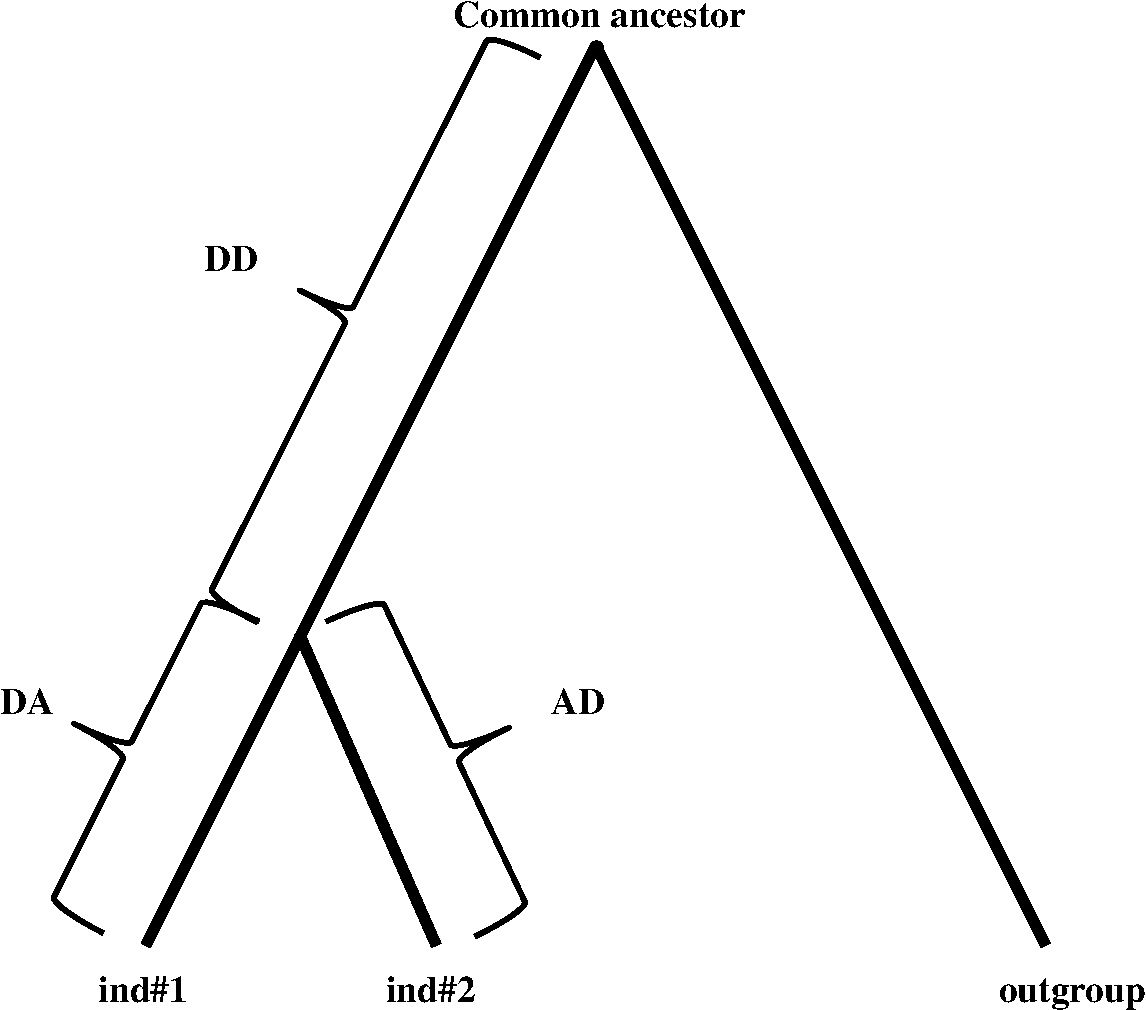
\includegraphics[width=0.5\textwidth,natwidth=510,natheight=542]{coasnowhite.eps}}
\caption{
While conditioning on bi-allelic segregating sites, glactools can compute the fraction of such sites that coalesce in the common lineage. If both individuals carry the derived allele, it is likely to coalesce in the common branch. The average coalescence for a given individual attempts to measure the fraction of sites that coalesce in the lineage specific to that individual.}
\label{fig:div}
\end{figure}

%\clearpage

The results are reported for each window. The last ``window'' are all the data with bootstraps. Each window contains the following category: all, onlyCpg, noCpg, transitions, transversions, noDamage.\\

Each category contains: absence of mutation ($AA$), mutation in the common branch ($DD$), mutation in branch for individual \#1 ($DA$), mutation in branch for individual \#2 ($AD$), $\frac { DA} { DA+DD }$, lower bound for $\frac { DA} { DA+DD }$, higher bound for $\frac { DA} { DA+DD }$, $\frac { AD} { AD+DD }$, lower bound for $\frac { AD} { AD+DD }$, higher bound for $\frac { AD} { AD+DD }$. If this is the last window with all the data with bootstraps, it also contains the mean from bootstraps, the standard deviation, $Z$ score.


To plot the output, 2 R scripts are available, one to make barplots:

\begin{lstlisting}
paircoacompute2barplot.R [output pairwise coa] [samples to include, comma delim] [ancient samples to exclude, comma delim] [pdf out]
\end{lstlisting}

another to make a heatmap:
\begin{lstlisting}
paircoacompute2heatmap.R [output pairwise coa] [samples to include, comma delim] [pdf out prefix] [pdf size]
\end{lstlisting}

You might have to tweek the fonts and margins. If you get a margin problem, use a large pdf size (e.g. 20).


\subsubsection{D-statistics}


In the previous section, we focused on sites where an allele could be parsimoniously traced to a given lineage. However, given three individuals where a third falls outside of the variation of the first two, there are cases where derived mutations in this third individual cannot be parsimoniously traced to a specific lineage 2 (see Figure \ref{fig:dstat}). More precisely, there are two possibilities: if the ind\#1 carries the derived allele but the other does not (DADA) or vice-versa (ADDA). In practice, such cases occur due to the existence of both alleles in both populations but where one was not sampled. However, in the absence of admixture or substructure, both cases are expected to occur with equal frequency. If admixture occurred between the third individual (labeled ``source'' in Figure \ref{fig:dstat}) and one of the first two (either ind\#1 or ind\#2), more derived alleles will be seen in that individual. The D-statistic (see \cite{patterson2012ancient}) attempts to measure imbalance between both cases by computing the following ratio:


\[
D= \frac {ADDA-DADA} {ADDA+DADA}
\]


If the result is close to 0, this can indicate a lack of greater proximity of one of the two individuals to the third one. To obtain a confidence score, we compute the D-statistics for bootstrap sets and compute the average D-statistics  ($\mu_{D_{boot}}$)) and the standard deviation ($\sigma_{D_{boot}}$). To assess the confidence score  we use the standard score ($Z$ ) as such:

\[
Z = \frac { D - \mu_{D_{boot}}  } {\sigma_{D_{boot}}}
\]


\begin{figure}[!tpb]%figure1
\centerline{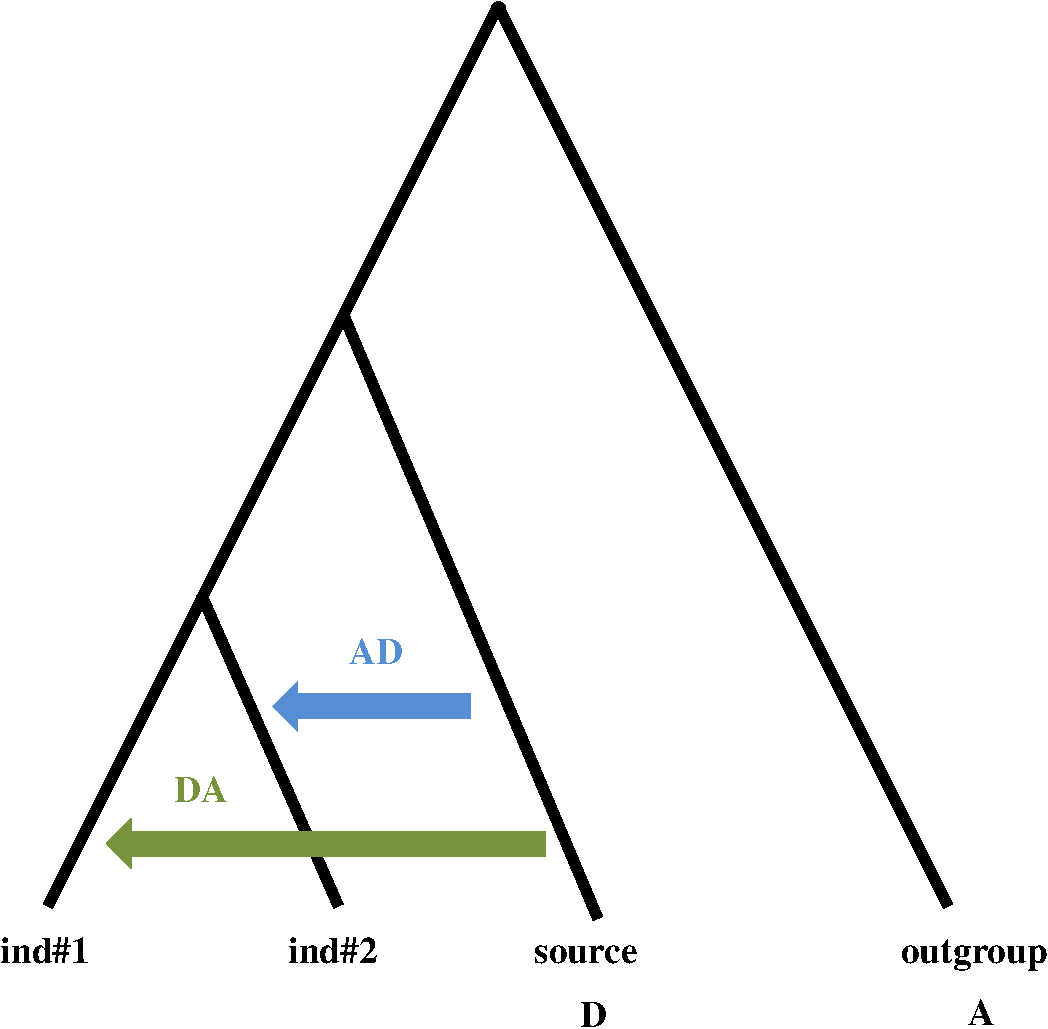
\includegraphics[width=0.5\textwidth,natwidth=510,natheight=542]{dstatnowhite.eps}}
\caption{Given gene flow, a certain individual will carry a greater proportion of derived alleles from the potential source.}
\label{fig:dstat}
\end{figure}

%\afterpage{\clearpage}
%

The results are reported for each window. The last ``window'' are all the data with bootstraps. Each window contains the following category: all, onlyCpg, noCpg, transitions, transversions, noDamage.\\

Each category contains: absence of mutation in both individuals ($AA$), individual \#1 has the ancestral allele but \#2 has the derived  ($AD$), individual \#1 has the derived allele but \#2 has the ancestral  ($DA$), absence of mutation in both individuals ($DD$),  $\frac {ADDA-DADA} {ADDA+DADA}$. If this is the last window (all the data plus bootstraps), it will also report next to the D-stats, the mean from bootstraps, the standard deviation from bootstraps, $Z$ score.



To plot the output, 2 R scripts are available, one to make barplots:

\begin{lstlisting}
dstats2pdf.R [dstat file] [output prefix pdf]
\end{lstlisting}

another to make a heatmap:
\begin{lstlisting}
dstats2heatmap.R [dstat file] [sample source] [pdf out prefix] [pdf size]
\end{lstlisting}

You might have to tweek the fonts and margins. If you get a margin problem, use a large pdf size (e.g. 20).




%\subsection{Unique of union}

%\noindent This program will print the unique union of the glac files to stdout. Used to merge the same files from different filters.

%\begin{lstlisting}
%uniq [glac file 1] [glac file 2] ...
%\end{lstlisting}






\newpage

\section{Exporting data}
\subsection{To BED}

To print an GLF/ACF as BED but where contiguous regions have been merged.
\begin{lstlisting}
glactools glac2bed  [options] <ACF/GLF file>
\end{lstlisting}


\subsection{To binary PLINK}

\noindent This program takes an ACF file and prints the genotype and SNP file in PLINK format

\tiny
\begin{lstlisting}
glactools acf2bplink  [options] <ACF file> [out prefix]
\end{lstlisting}
\normalsize

\subsection{To FASTA}

\noindent This program takes an ACF file and prints a FASTA file using the allele information with one record per population. Each site generates one base pair.

\begin{lstlisting}
glactools acf2fasta  [options] <ACF file>
\end{lstlisting}


\subsection{To G-PhoCS}

\noindent This program takes an ACF file and prints G-Phocs output given a certain range specified in a BED file.

\begin{lstlisting}
glactools acf2ghocs  [options]  <ACF file> <bedfile>
\end{lstlisting}

We recommend using glac2gphocsWrapper.pl is this automates the process and calls ``glac2bed'' for you.

\subsection{To NEXUS}

\noindent This program takes an ACF matrix and prints the alleles in NEXUS format.

\begin{lstlisting}
glactools acf2nexus [options] <ACF file> 
\end{lstlisting}

\subsection{To EIGENSTRAT}
\noindent This program takes an ACF file and exports the data in EIGENSTRAT.
\tiny
\begin{lstlisting}
glactools acf2eigenstrat  [options] <ACF file> [out prefix]
\end{lstlisting}
\normalsize

\subsection{To Treemix}

To print Treemix input.
\begin{lstlisting}
glactools acf2treemix  [options] <ACF file>
\end{lstlisting}






%\lipsum




\newpage


%%%%%%%%%%%%%%%%%%%%%%%%%%%%%%%%%%%%%%%%%%%%%%%%%%%%%%%%%%%%%%%%%%%%


%%%%%%%%%%%%%%%%%%%%%%%%%%%%%%%%%%%%%%%%%%%%%%%%%%%%%%%%%%%%%%%%%%%%%%

%\input lay_e2

%%%%%%%%%%%%%%%%%%%%%%%%%%%%%%%%%%%%%%%%%%%%%%%%%%%%%%%%%%%%%%%%%%%%%%

\bibliographystyle{plainnat}
\bibliography{bibli.bib} 


\end{document}
